\documentclass[aspectratio=169]{beamer}

%\documentclass[handout]{beamer}
%% To make 4 per page
%\usepackage{pgfpages}
%\mode<handout>{\setbeamercolor{background canvas}{bg=white}}
%\pgfpagesuselayout{4 on 1}[letterpaper,landscape]%,border shrink=5mm]

\usetheme{default}
% Slide setup, colour independent

\usepackage{amsmath,amssymb,amsthm}
\usepackage{colortbl}
\usepackage{bm}
\usepackage{xcolor}
\usepackage{dsfont}
\usepackage{setspace}
%\usepackage{subfigure}
% To use \ding{234} and the like
\usepackage{pifont}
% To cross reference between slide files
\usepackage{zref-xr,zref-user}
% Use something like
% \zexternaldocument{fileI}
% in the tex files. And cite using \zref instead of \ref

% Fields and the like
\def\IC{\mathbb{C}}
\def\IF{\mathbb{F}}
\def\II{\mathbb{I}}
\def\IJ{\mathbb{J}}
\def\IM{\mathbb{M}}
\def\IN{\mathbb{N}}
\def\IP{\mathbb{P}}
\def\IR{\mathbb{R}}
\def\IZ{\mathbb{Z}}
\def\11{\mathds{1}}


% Bold lowercase
\def\ba{\mathbf{a}}
\def\bb{\mathbf{b}}
\def\bc{\mathbf{c}}
\def\bd{\mathbf{d}}
\def\be{\mathbf{e}}
\def\bf{\mathbf{f}}
\def\bh{\mathbf{h}}
\def\bi{\mathbf{i}}
\def\bj{\mathbf{j}}
\def\bk{\mathbf{k}}
\def\bn{\mathbf{n}}
\def\bp{\mathbf{p}}
\def\br{\mathbf{r}}
\def\bs{\mathbf{s}}
\def\bu{\mathbf{u}}
\def\bv{\mathbf{v}}
\def\bw{\mathbf{w}}
\def\bx{\mathbf{x}}
\def\by{\mathbf{y}}
\def\bz{\mathbf{z}}

% Bold capitals
\def\bB{\mathbf{B}}
\def\bD{\mathbf{D}}
\def\bF{\mathbf{F}}
\def\bG{\mathbf{G}}
\def\bI{\mathbf{I}}
\def\bL{\mathbf{L}}
\def\bN{\mathbf{N}}
\def\bP{\mathbf{P}}
\def\bR{\mathbf{R}}
\def\bS{\mathbf{S}}
\def\bT{\mathbf{T}}
\def\bX{\mathbf{X}}

% Bold numbers
\def\b0{\mathbf{0}}

% Bold greek
\bmdefine{\bmu}{\bm{\mu}}
\def\bphi{\bm{\phi}}
\def\bvarphi{\bm{\varphi}}

% Bold red sentence
\def\boldred#1{{\color{red}\textbf{#1}}}
\def\defword#1{{\color{orange}\textbf{#1}}}

% Caligraphic letters
\def\A{\mathcal{A}}
\def\B{\mathcal{B}}
\def\C{\mathcal{C}}
\def\D{\mathcal{D}}
\def\E{\mathcal{E}}
\def\F{\mathcal{F}}
\def\G{\mathcal{G}}
\def\H{\mathcal{H}}
\def\I{\mathcal{I}}
\def\L{\mathcal{L}}
\def\M{\mathcal{M}}
\def\N{\mathcal{N}}
\def\P{\mathcal{P}}
\def\R{\mathcal{R}}
\def\S{\mathcal{S}}
\def\T{\mathcal{T}}
\def\U{\mathcal{U}}
\def\V{\mathcal{V}}

% tt font for code
\def\code#1{{\tt #1}}

% i.e., e.g.
\def\eg{\emph{e.g.}}
\def\ie{\emph{i.e.}}


% Operators and special symbols
\def\nbOne{{\mathchoice {\rm 1\mskip-4mu l} {\rm 1\mskip-4mu l}
{\rm 1\mskip-4.5mu l} {\rm 1\mskip-5mu l}}}
\def\cov{\ensuremath{\mathsf{cov}}}
\def\Var{\ensuremath{\mathsf{Var}\ }}
\def\Im{\textrm{Im}\;}
\def\Re{\textrm{Re}\;}
\def\det{\ensuremath{\mathsf{det}}}
\def\diag{\ensuremath{\mathsf{diag}}}
\def\nullspace{\ensuremath{\mathsf{null}}}
\def\nullity{\ensuremath{\mathsf{nullity}}}
\def\rank{\ensuremath{\mathsf{rank}}}
\def\range{\ensuremath{\mathsf{range}}}
\def\sgn{\ensuremath{\mathsf{sgn}}}
\def\Span{\ensuremath{\mathsf{span}}}
\def\tr{\ensuremath{\mathsf{tr}}}
\def\imply{$\Rightarrow$}
\def\restrictTo#1#2{\left.#1\right|_{#2}}
\newcommand{\parallelsum}{\mathbin{\!/\mkern-5mu/\!}}
\def\dsum{\mathop{\displaystyle \sum }}%
\def\dind#1#2{_{\substack{#1\\ #2}}}

\DeclareMathOperator{\GL}{GL}
\DeclareMathOperator{\Rel}{Re}
\def\Nt#1{\left|\!\left|\!\left|#1\right|\!\right|\!\right|}
\newcommand{\tripbar}{|\! |\! |}



% The beamer bullet (in base colour)
\def\bbullet{\leavevmode\usebeamertemplate{itemize item}\ }

% Theorems and the like
\newtheorem{proposition}[theorem]{Proposition}
\newtheorem{property}[theorem]{Property}
\newtheorem{importantproperty}[theorem]{Property}
\newtheorem{importanttheorem}[theorem]{Theorem}
%\newtheorem{lemma}[theorem]{Lemma}
%\newtheorem{corollary}[theorem]{Corollary}
\newtheorem{remark}[theorem]{Remark}
\setbeamertemplate{theorems}[numbered]
%\setbeamertemplate{theorems}[ams style]

%
%\usecolortheme{orchid}
%\usecolortheme{orchid}

\def\red{\color[rgb]{1,0,0}}
\def\blue{\color[rgb]{0,0,1}}
\def\green{\color[rgb]{0,1,0}}


% Get rid of navigation stuff
\setbeamertemplate{navigation symbols}{}

% Set footline/header line
\setbeamertemplate{footline}
{%
\quad p. \insertpagenumber \quad--\quad \insertsection\vskip2pt
}
% \setbeamertemplate{headline}
% {%
% \quad\insertsection\hfill p. \insertpagenumber\quad\mbox{}\vskip2pt
% }


\makeatletter
\newlength\beamerleftmargin
\setlength\beamerleftmargin{\Gm@lmargin}
\makeatother

% Colours for special pages
\def\extraContent{yellow!20}


%%%%%%%%%%%%%%%%%
\usepackage{tikz}
\usetikzlibrary{shapes,arrows}
\usetikzlibrary{positioning}
\usetikzlibrary{shapes.symbols,shapes.callouts,patterns}
\usetikzlibrary{calc,fit}
\usetikzlibrary{backgrounds}
\usetikzlibrary{decorations.pathmorphing,fit,petri}
\usetikzlibrary{automata}
\usetikzlibrary{fadings}
\usetikzlibrary{patterns,hobby}

\usetikzlibrary{backgrounds,fit,petri}


\usepackage{pgfplots}
\pgfplotsset{compat=1.6}
\pgfplotsset{ticks=none}

\usetikzlibrary{decorations.markings}
\usetikzlibrary{arrows.meta}
\tikzset{>=stealth}

% For tikz
\usetikzlibrary{shapes,arrows}
\usetikzlibrary{positioning}
\tikzstyle{cloud} = [draw, ellipse,fill=red!20, node distance=0.87cm,
minimum height=2em]
\tikzstyle{line} = [draw, -latex']


%%% For max frame images
\newenvironment{changemargin}[2]{%
\begin{list}{}{%
\setlength{\topsep}{0pt}%
\setlength{\leftmargin}{#1}%
\setlength{\rightmargin}{#2}%
\setlength{\listparindent}{\parindent}%
\setlength{\itemindent}{\parindent}%
\setlength{\parsep}{\parskip}%
}%
\item[]}{\end{list}}


% Make one image take up the entire slide content area in beamer,.:
% centered/centred full-screen image, with title:
% This uses the whole screen except for the 1cm border around it
% all. 128x96mm
\newcommand{\titledFrameImage}[2]{
\begin{frame}{#1}
%\begin{changemargin}{-1cm}{-1cm}
\begin{center}
\includegraphics[width=108mm,height=\textheight,keepaspectratio]{#2}
\end{center}
%\end{changemargin}
\end{frame}
}

% Make one image take up the entire slide content area in beamer.:
% centered/centred full-screen image, no title:
% This uses the whole screen except for the 1cm border around it
% all. 128x96mm
\newcommand{\plainFrameImage}[1]{
\begin{frame}[plain]
%\begin{changemargin}{-1cm}{-1cm}
\begin{center}
\includegraphics[width=108mm,height=76mm,keepaspectratio]{#1}
\end{center}
%\end{changemargin}
\end{frame}
}

% Make one image take up the entire slide area, including borders, in beamer.:
% centered/centred full-screen image, no title:
% This uses the entire whole screen
\newcommand{\maxFrameImage}[1]{
\begin{frame}[plain]
\begin{changemargin}{-1cm}{-1cm}
\begin{center}
\includegraphics[width=\paperwidth,height=\paperheight,keepaspectratio]
{#1}
\end{center}
\end{changemargin}
\end{frame}
}

% This uses the entire whole screen (to include in frame)
\newcommand{\maxFrameImageNoFrame}[1]{
\begin{changemargin}{-1cm}{-1cm}
\begin{center}
\includegraphics[width=\paperwidth,height=0.99\paperheight,keepaspectratio]
{#1}
\end{center}
\end{changemargin}
}

% Make one image take up the entire slide area, including borders, in beamer.:
% centered/centred full-screen image, no title:
% This uses the entire whole screen
\newcommand{\maxFrameImageColor}[2]{
\begin{frame}[plain]
\setbeamercolor{normal text}{bg=#2!20}
\begin{changemargin}{-1cm}{-1cm}
\begin{center}
\includegraphics[width=\paperwidth,height=\paperheight,keepaspectratio]
{#1}
\end{center}
\end{changemargin}
\end{frame}
}


\usepackage{tikz}
\usetikzlibrary{patterns,hobby}
\usepackage{pgfplots}
\pgfplotsset{compat=1.6}
\pgfplotsset{ticks=none}

\usetikzlibrary{backgrounds}
\usetikzlibrary{decorations.markings}
\usetikzlibrary{arrows.meta}
\tikzset{>=stealth}

\tikzset{
  clockwise arrows/.style={
    postaction={
      decorate,
      decoration={
        markings,
        mark=between positions 0.1 and 0.9 step 40pt with {\arrow{>}},
   }}}}


   %%%%%%%%%%%
% To have links to parts in the outline
\makeatletter
\AtBeginPart{%
  \addtocontents{toc}{\protect\beamer@partintoc{\the\c@part}{\beamer@partnameshort}{\the\c@page}}%
}
%% number, shortname, page.
\providecommand\beamer@partintoc[3]{%
  \ifnum\c@tocdepth=-1\relax
    % requesting onlyparts.
    \makebox[6em]{Part #1:} \textcolor{green!30!blue}{\hyperlink{#2}{#2}}
    \par
  \fi
}
\define@key{beamertoc}{onlyparts}[]{%
  \c@tocdepth=-1\relax
}
\makeatother%

\newcommand{\nameofthepart}{}
\newcommand{\nupart}[1]%
    {   \part{#1}%
        \renewcommand{\nameofthepart}{#1}%
        {
          \setbeamercolor{background canvas}{bg=orange!50}
          \begin{frame}{#1}%\partpage 
          \hypertarget{\nameofthepart}{}\tableofcontents%
          \end{frame}
        }
    }



\usecolortheme{orchid}

%% Listings
\usepackage{listings}
\definecolor{mygreen}{rgb}{0,0.6,0}
\definecolor{mygray}{rgb}{0.5,0.5,0.5}
\definecolor{mymauve}{rgb}{0.58,0,0.82}
\definecolor{mygold}{rgb}{1,0.843,0}
\definecolor{myblue}{rgb}{0.537,0.812,0.941}

\definecolor{lgreen}{rgb}{0.6,0.9,.6}
\definecolor{lred}{rgb}{1,0.5,.5}

\lstloadlanguages{R}
\lstset{ %
  language=R,
  backgroundcolor=\color{black!05},   % choose the background color
  basicstyle=\footnotesize\ttfamily,        % size of fonts used for the code
  breaklines=true,                 % automatic line breaking only at whitespace
  captionpos=b,                    % sets the caption-position to bottom
  commentstyle=\color{mygreen},    % comment style
  escapeinside={\%*}{*)},          % if you want to add LaTeX within your code
  keywordstyle=\color{red},       % keyword style
  stringstyle=\color{mygold},     % string literal style
  keepspaces=true,
  columns=fullflexible,
  tabsize=4,
}
% Could also do (in lstset)
% basicstyle==\fontfamily{pcr}\footnotesize
\lstdefinelanguage{Renhanced}%
  {keywords={abbreviate,abline,abs,acos,acosh,action,add1,add,%
      aggregate,alias,Alias,alist,all,anova,any,aov,aperm,append,apply,%
      approx,approxfun,apropos,Arg,args,array,arrows,as,asin,asinh,%
      atan,atan2,atanh,attach,attr,attributes,autoload,autoloader,ave,%
      axis,backsolve,barplot,basename,besselI,besselJ,besselK,besselY,%
      beta,binomial,body,box,boxplot,break,browser,bug,builtins,bxp,by,%
      c,C,call,Call,case,cat,category,cbind,ceiling,character,char,%
      charmatch,check,chol,chol2inv,choose,chull,class,close,cm,codes,%
      coef,coefficients,co,col,colnames,colors,colours,commandArgs,%
      comment,complete,complex,conflicts,Conj,contents,contour,%
      contrasts,contr,control,helmert,contrib,convolve,cooks,coords,%
      distance,coplot,cor,cos,cosh,count,fields,cov,covratio,wt,CRAN,%
      create,crossprod,cummax,cummin,cumprod,cumsum,curve,cut,cycle,D,%
      data,dataentry,date,dbeta,dbinom,dcauchy,dchisq,de,debug,%
      debugger,Defunct,default,delay,delete,deltat,demo,de,density,%
      deparse,dependencies,Deprecated,deriv,description,detach,%
      dev2bitmap,dev,cur,deviance,off,prev,,dexp,df,dfbetas,dffits,%
      dgamma,dgeom,dget,dhyper,diag,diff,digamma,dim,dimnames,dir,%
      dirname,dlnorm,dlogis,dnbinom,dnchisq,dnorm,do,dotplot,double,%
      download,dpois,dput,drop,drop1,dsignrank,dt,dummy,dump,dunif,%
      duplicated,dweibull,dwilcox,dyn,edit,eff,effects,eigen,else,%
      emacs,end,environment,env,erase,eval,equal,evalq,example,exists,%
      exit,exp,expand,expression,External,extract,extractAIC,factor,%
      fail,family,fft,file,filled,find,fitted,fivenum,fix,floor,for,%
      For,formals,format,formatC,formula,Fortran,forwardsolve,frame,%
      frequency,ftable,ftable2table,function,gamma,Gamma,gammaCody,%
      gaussian,gc,gcinfo,gctorture,get,getenv,geterrmessage,getOption,%
      getwd,gl,glm,globalenv,gnome,GNOME,graphics,gray,grep,grey,grid,%
      gsub,hasTsp,hat,heat,help,hist,home,hsv,httpclient,I,identify,if,%
      ifelse,Im,image,\%in\%,index,influence,measures,inherits,install,%
      installed,integer,interaction,interactive,Internal,intersect,%
      inverse,invisible,IQR,is,jitter,kappa,kronecker,labels,lapply,%
      layout,lbeta,lchoose,lcm,legend,length,levels,lgamma,library,%
      licence,license,lines,list,lm,load,local,locator,log,log10,log1p,%
      log2,logical,loglin,lower,lowess,ls,lsfit,lsf,ls,machine,Machine,%
      mad,mahalanobis,make,link,margin,match,Math,matlines,mat,matplot,%
      matpoints,matrix,max,mean,median,memory,menu,merge,methods,min,%
      missing,Mod,mode,model,response,mosaicplot,mtext,mvfft,na,nan,%
      names,omit,nargs,nchar,ncol,NCOL,new,next,NextMethod,nextn,%
      nlevels,nlm,noquote,NotYetImplemented,NotYetUsed,nrow,NROW,null,%
      numeric,\%o\%,objects,offset,old,on,Ops,optim,optimise,optimize,%
      options,or,order,ordered,outer,package,packages,page,pairlist,%
      pairs,palette,panel,par,parent,parse,paste,path,pbeta,pbinom,%
      pcauchy,pchisq,pentagamma,persp,pexp,pf,pgamma,pgeom,phyper,pico,%
      pictex,piechart,Platform,plnorm,plogis,plot,pmatch,pmax,pmin,%
      pnbinom,pnchisq,pnorm,points,poisson,poly,polygon,polyroot,pos,%
      postscript,power,ppoints,ppois,predict,preplot,pretty,Primitive,%
      print,prmatrix,proc,prod,profile,proj,prompt,prop,provide,%
      psignrank,ps,pt,ptukey,punif,pweibull,pwilcox,q,qbeta,qbinom,%
      qcauchy,qchisq,qexp,qf,qgamma,qgeom,qhyper,qlnorm,qlogis,qnbinom,%
      qnchisq,qnorm,qpois,qqline,qqnorm,qqplot,qr,Q,qty,qy,qsignrank,%
      qt,qtukey,quantile,quasi,quit,qunif,quote,qweibull,qwilcox,%
      rainbow,range,rank,rbeta,rbind,rbinom,rcauchy,rchisq,Re,read,csv,%
      csv2,fwf,readline,socket,real,Recall,rect,reformulate,regexpr,%
      relevel,remove,rep,repeat,replace,replications,report,require,%
      resid,residuals,restart,return,rev,rexp,rf,rgamma,rgb,rgeom,R,%
      rhyper,rle,rlnorm,rlogis,rm,rnbinom,RNGkind,rnorm,round,row,%
      rownames,rowsum,rpois,rsignrank,rstandard,rstudent,rt,rug,runif,%
      rweibull,rwilcox,sample,sapply,save,scale,scan,scan,screen,sd,se,%
      search,searchpaths,segments,seq,sequence,setdiff,setequal,set,%
      setwd,show,sign,signif,sin,single,sinh,sink,solve,sort,source,%
      spline,splinefun,split,sqrt,stars,start,stat,stem,step,stop,%
      storage,strstrheight,stripplot,strsplit,structure,strwidth,sub,%
      subset,substitute,substr,substring,sum,summary,sunflowerplot,svd,%
      sweep,switch,symbol,symbols,symnum,sys,status,system,t,table,%
      tabulate,tan,tanh,tapply,tempfile,terms,terrain,tetragamma,text,%
      time,title,topo,trace,traceback,transform,tri,trigamma,trunc,try,%
      ts,tsp,typeof,unclass,undebug,undoc,union,unique,uniroot,unix,%
      unlink,unlist,unname,untrace,update,upper,url,UseMethod,var,%
      variable,vector,Version,vi,warning,warnings,weighted,weights,%
      which,while,window,write,\%x\%,x11,X11,xedit,xemacs,xinch,xor,%
      xpdrows,xy,xyinch,yinch,zapsmall,zip},%
   otherkeywords={!,!=,~,$,*,\%,\&,\%/\%,\%*\%,\%\%,<-,<<-,_,/},%
   alsoother={._$},%
   sensitive,%
   morecomment=[l]\#,%
   morestring=[d]",%
   morestring=[d]'% 2001 Robert Denham
  }%

%%%%%%% 
%% Definitions in yellow boxes
\usepackage{etoolbox}
\setbeamercolor{block title}{use=structure,fg=structure.fg,bg=structure.fg!40!bg}
\setbeamercolor{block body}{parent=normal text,use=block title,bg=block title.bg!20!bg}

\BeforeBeginEnvironment{definition}{%
	\setbeamercolor{block title}{fg=black,bg=yellow!20!white}
	\setbeamercolor{block body}{fg=black, bg=yellow!05!white}
}
\AfterEndEnvironment{definition}{
	\setbeamercolor{block title}{use=structure,fg=structure.fg,bg=structure.fg!20!bg}
	\setbeamercolor{block body}{parent=normal text,use=block title,bg=block title.bg!50!bg, fg=black}
}
\BeforeBeginEnvironment{importanttheorem}{%
	\setbeamercolor{block title}{fg=black,bg=red!20!white}
	\setbeamercolor{block body}{fg=black, bg=red!05!white}
}
\AfterEndEnvironment{importanttheorem}{
	\setbeamercolor{block title}{use=structure,fg=structure.fg,bg=structure.fg!20!bg}
	\setbeamercolor{block body}{parent=normal text,use=block title,bg=block title.bg!50!bg, fg=black}
}
\BeforeBeginEnvironment{importantproperty}{%
	\setbeamercolor{block title}{fg=black,bg=red!50!white}
	\setbeamercolor{block body}{fg=black, bg=red!30!white}
}
\AfterEndEnvironment{importantproperty}{
	\setbeamercolor{block title}{use=structure,fg=structure.fg,bg=structure.fg!20!bg}
	\setbeamercolor{block body}{parent=normal text,use=block title,bg=block title.bg!50!bg, fg=black}
}


% Beginning of a section
\AtBeginSection[]{
	{
		\setbeamercolor{background canvas}{bg=yellow!10}
		\begin{frame}[noframenumbering,plain]
			\framesubtitle{\nameofthepart Chapter \insertromanpartnumber \ -- \iteminsert{\insertpart}}
			\tableofcontents[
				currentsection,
				sectionstyle=show/shaded,
				subsectionstyle=show/show/hide]
		\end{frame}
	\addtocounter{page}{-1}
	%\addtocounter{framenumber}{-1} 
	}
}

% Beginning of a section
\AtBeginSubsection[]{
	{
		\setbeamercolor{background canvas}{bg=green!10}
		\begin{frame}[noframenumbering,plain]
				\framesubtitle{\nameofthepart Chapter \insertromanpartnumber \ -- \iteminsert{\insertpart}}
				\tableofcontents[
					currentsection,
					sectionstyle=show/show,
					currentsubsection,
					subsectionstyle=show/shaded/hide]
			\end{frame}
		\addtocounter{page}{-1}
	}
}


% To have theorems and everything derived prefixed by the slide set
% number
\renewcommand{\thetheorem}{4.\arabic{theorem}}



\title{Factorisations, canonical forms and decompositions}
\author{Julien Arino}
\date{Fall 2023}

%%%%%%%%%%%%%%%%%%%%%
%%%%%%%%%%%%%%%%%%%%%
%%%%%%%%%%%%%%%%%%%%%
%%%%%%%%%%%%%%%%%%%%%
%%%%%%%%%%%%%%%%%%%%%
%%%%%%%%%%%%%%%%%%%%%
%%%%%%%%%%%%%%%%%%%%%
%%%%%%%%%%%%%%%%%%%%%
\begin{document}

% The title page
\begin{frame}[noframenumbering,plain]
  \begin{tikzpicture}[remember picture,overlay]
    \node[above right,inner sep=0pt] at (current page.south west)
    {
        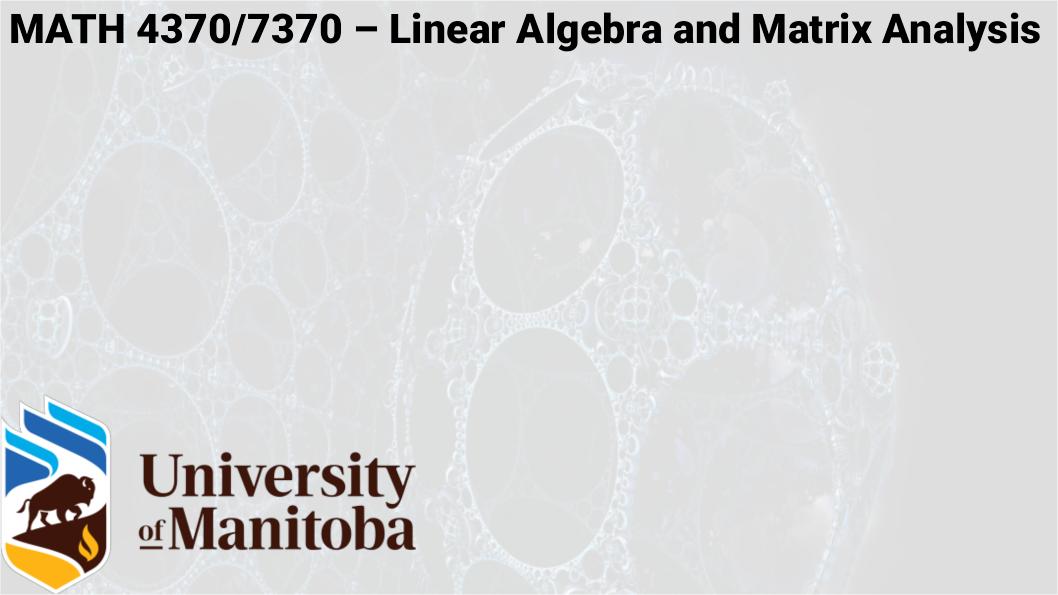
\includegraphics[width=\paperwidth]{title-page-picture.png}
    };
\end{tikzpicture}
	\titlepage
\end{frame}
\addtocounter{page}{-1}
  
  
\begin{frame}{Outline}
	  \tableofcontents[hideallsubsections]
\end{frame}
\addtocounter{page}{-1}


%%%%%%%%%%%%%%%%%%%%%%%%%%%
%%%%%%%%%%%%%%%%%%%%%%%%%%%
%%%%%%%%%%%%%%%%%%%%%%%%%%%
%%%%%%%%%%%%%%%%%%%%%%%%%%%
\section{Unitary matrices and QR factorisation}

\begin{frame}
\begin{definition}
Let $\bx_1, \ldots, \bx_k\in \IC^n$. We say that $\bx_1, \ldots, \bx_k$ is an \defword{orthogonal list} if $\bx_i^*\bx_j=0$ for all $i \neq j$. If, in addition, we have that $\bx_i^*\bx_i=1$, then we say that the list is \defword{orthonormal}
\end{definition}
\vfill
\begin{theorem}\label{th:every_ortho_list_is)LI}
Every orthonormal list of vectors in $\IC^n$ is linearly independent
\end{theorem}
\vfill
\begin{remark}
In Theorem~\ref{th:every_ortho_list_is)LI}, if we have ``only'' orthogonal vectors, we need to replace ``list of vectors'' by ``list of non-zero vectors'' in the statement 
\end{remark}
\end{frame}


\begin{frame}
\begin{definition}
Let $U\in \mathcal{M}_n$, we say that $U$ is an \defword{unitary matrix} if $U^*U=\II$. Furthermore, we say that $U\in \mathcal{M}_n(\IR)$ is a \defword{(real) orthogonal matrix} if $U^TU=\II$
\end{definition}
\vfill
\begin{theorem}
 Let $U\in \mathcal{M}_n$. TFAE:
 \begin{enumerate}
     \item $U$ is unitary
     \item $U$ is non-singular and $U^*=U^{-1}$
     \item $UU^*=\II$
     \item $U^*$ is unitary
     \item the columns of $U$ are orthonormal
     \item the rows of $U$ are orthonormal
     \item for all $\bx\in \IC^n$ we have $\|\bx\|_2= \|U\bx\|_2$
 \end{enumerate}
\end{theorem}
\end{frame}

\begin{frame}
\begin{definition}
A \defword{linear transformation} $T: \IC^n \to \IC^n$ is a \defword{Euclidean isometry} if $\|\bx\|_2= \| T\bx \|_2$ for all $\bx\in \IC^n$ 
\end{definition}
\vfill
\begin{corollary}
Let $U \in \mathcal{M}_n$. $U$ is a Euclidean isometry if and only if $U$ is unitary
\end{corollary}
\end{frame}



\begin{frame}
\begin{remark}
Let $U,\, V\in \mathcal{M}_n$ are unitary matrices (respectively real orthogonal), then $UV$ is unitary (respectively real orthogonal).

Indeed, $U,V$ unitary $\Leftrightarrow$ $U^{-1},V^{-1}$ exist and $U^{-1}=U^*,V^{-1}=V^*$. Then
\begin{align*}
UV\textrm{ unitary } &\Leftrightarrow (UV)^*UV=\II \\
&\Leftrightarrow V^*U^*UV=\II \\
&\Leftrightarrow \II = \II
\end{align*}
\end{remark}
\vfill
\textbf{Notation}: $\GL(n, \IF)$ is the general linear group, where the elements are non-singular matrices in $\mathcal{M}_n(\IF)$
\end{frame}


\begin{frame}
\begin{theorem}
 The set of unitary (respectively real orhogonal) matrices in $\mathcal{M}_n$ forms a group, the $n\times n$ unitary (respectively real orthogonal) subgroup of $\GL(n,\, \IC)$ (respectively $\GL(n,\, \IR)$)
\end{theorem}
\vfill
\begin{theorem}[Selection Principle]
Suppose that we have a sequence of unitary matrices $U_1, U_2 \ldots, \in \mathcal{M}_n$. Then there exists a subsequence $U_{k_1}, U_{k_2}\ldots $ such that the entries of $U_{k_i}$ converge to entries of a unitary matrix as $i\to \infty$
\end{theorem}
\end{frame}


\begin{frame}
\begin{lemma}
Let $U\in \mathcal{M}_n$ be a unitary matrix partitioned as 
\[U=\begin{pmatrix}
U_{11}& U_{12}\\
U_{21}& U_{22}
\end{pmatrix},\]
with $U_{ii}\in \mathcal{M}_k$. Then $\rank U_{12}= \rank U_{21}$ and $\rank U_{22}=\rank U_{11}+n -2k$. If, furthermore, $U_{21}=0$ and $U_{12}=0$, then $U_{11}$ and $U_{22}$ are unitary
\end{lemma}
\end{frame}


\begin{frame}
\begin{theorem}[QR factorisation]
 Let $A\in \mathcal{M}_{nm}$
 \begin{enumerate}
     \item If $n \geq m$, there is a $Q\in \mathcal{M}_{nm}$ with orthogonormal columns and upper triangular $R\in \mathcal{M}_m$ with non-negative main diaginal entries such that $A=QR$
     \item If $\rank A=m $  then the factors $Q$ and $R$ in (1) are uniquely determined and the main diagonal entries of R are all positive
     \item If $n=m$, Then the factor $Q$ in (1) is unitary
     \item There is a unitary $Q \in  \mathcal{M}_n$ and an upper triangular $R \in  \mathcal{M}_{nm}$ with nonnegative diagonal entries such that $A = Q R$
     \item If $A$ is real, then $Q$ and $R$ are in (1), (2), (3), and (4) may be taken to be real
 \end{enumerate}
\end{theorem}
\end{frame}

%%%%%%%%%%%%%%%%%%%%%%%%%%%
%%%%%%%%%%%%%%%%%%%%%%%%%%%
%%%%%%%%%%%%%%%%%%%%%%%%%%%
%%%%%%%%%%%%%%%%%%%%%%%%%%%
\section{Schur's Form }


\begin{frame}
For a unitary matrix $U$, $U^*=U$, so the transformation $A\mapsto U^*AU$ is a \defword{similarity transformation}, provided that $U$ is unitary. This is a \defword{unitary similarity}
\vfill
\begin{definition}[Unitarily similar matrices]
Let $A,\, B\in \mathcal{M}_n$. We say that $A$ is \defword{unitarily similar} to $B$ if there exists $U\in \mathcal{M}_n$ unitary such that 
\[
	A=U^*BU
\]
If $U$ can be taken real (i.e., if $U$ is real orthogonal) than $A$ is real orthogonal similar to $B$ (if $A=U^TBU$)
\end{definition}
\end{frame}


\begin{frame}
\begin{remark}
\begin{enumerate}
    \item Unitary similarity is an equivalence relation
    \item Unitary similarity implies similarity. However, the converse is not true
    \item Similarity is a change of bases. Unitary similarity is a change of orthonormal bases
\end{enumerate}
\end{remark}
\vfill
\begin{definition}[Householder matrix] Let $0 \neq \omega \in \IC^n$. The Householder matrix $U_{\omega}\in \mathcal{M}_n$ is 
\[
    U_{\omega}= \mathbb{I}-2(\omega^* \omega)^{-1} \omega \omega^*
\]
\end{definition}
\end{frame}

\begin{frame}
\begin{remark}
\begin{enumerate}
    \item If $\| \omega \|=1$ then $U_{\omega} = \mathbb{I}-2\omega\omega^*$
    \item Householder matrix are unitary and Hermitian, thus $U_{\omega}^{-1}= U_{\omega}$.
    \item The eigenvalues of a Householder matrix are $-1, 1, \ldots, 1$ and $| U_{\omega}|=1$
\end{enumerate}
\end{remark}
\end{frame}

\begin{frame}
\begin{theorem}
 Let $\bx,\by\in \IC^n$ and assume that $\|\bx\|_2= \|\by\|_2> 0$ 
 \begin{itemize}
     \item  If $\by=e^{i \theta}\bx$ for some $\theta\in \IR$ [$\bx,\by$ are linearly dependent], define $U(\by,\bx)= e^{i\theta}\II$
     \item Otherwise, let $\phi\in [0,\, 2\pi)$ be such that $\bx^*\by= e^{i\phi} |\bx^{*}\by|$ (taking $\phi=0$ if $\bx^*\by=0)$. Let $\omega= e^{i\phi}\bx-\by$ and define 
     \[
        U(\by,\bx)= e^{i\phi}U_{\omega}
    \]
     where $U_{\omega}= \mathbb{I}-2(\omega^* \omega)^{-1} \omega \omega^*$ is Householder
\end{itemize}
\begin{enumerate}
    \item $U(\by,\bx)$ unitary and essentially Hermitian
    \item $U(\by,\bx)\bx=\by$
    \item $U(\by,\bx)\bz \perp\by$, when $\bz\perp\by$
    \item If $\bx,\by\in \IR^n$, then $U(\by,\bx)$ is real and $U(\by,\bx)= \II$ if $\by=\bx$ and $U(\by,\bx)=U_{\bx-\by}\in \mathcal{M}_n(\IR)$ otherwise
\end{enumerate}
\end{theorem}
\end{frame}



\begin{frame}
\begin{remark}
For all $A\in \mathcal{M}_n$, $U(y,\,x)^*AU(y,\,x)= U_{\omega}^*AU_{\omega}$. This is called a Householder transformation.
\end{remark}
\vfill
\begin{theorem}[Schur's Form]
Let $A\in \mathcal{M}_n$ with eigenvalues $\lambda_1,\ldots, \lambda_n$ in any prescribed order (including multiplicities). Let $x\in \IC^n$, $\| x\|=1$, be such that $Ax= \lambda_1 x $
\begin{enumerate}
    \item There exists $U=[ x \, u_2 \ldots u_n]\in \mathcal{M}_n$ unitary such that $U^{*} AU= T$, where $T$ is upper triangular such that $t_ii= \lambda_i$, $i= 1, \ldots,n$. 
    \item If $A\in \mathcal{M}_n(\IR)$ and has real eigenvalues, then $x$ can be chosen to be real and there exists 
    \[Q=[ x \, q_2 \ldots q_n]\in \mathcal{M}_n(\IR)\]
    real orthogonal and such that $Q^TAQ=T$, with $T$ upper triangular with $t_{ii}=\lambda_1$ $i= 1, \ldots, n$. 
\end{enumerate}
\end{theorem}
\end{frame}


\begin{frame}
\begin{theorem}[Schur version 2]
Let $A\in \mathcal{M}_n$ with eigenvalues $\lambda_1, \ldots, \lambda_n$ (including mutiplicities). Then there esists $U\in \mathcal{M}_n$ such that 
\[U^* AU = \begin{pmatrix}
\lambda_1& * & \ldots &*\\
0 & \lambda_2& & \vdots\\
0&  &\ddots& * \\
0&& & \lambda_n
\end{pmatrix}\]
\end{theorem}
\vfill
\begin{remark}
The decomposition is not unique
\end{remark}
\end{frame}

\begin{frame}
\begin{theorem}
Let $U\in \mathcal{M}_n, A,\, B\in \mathcal{M}_n$. Suppose $A$ is unitarily similar to $B$, then 
\[\sum\limits_{i,\,j=1}^n | a_{ij}|^2= \sum\limits_{i,\, j}|b_{ij}|^2\]
\end{theorem}
\vfill
\begin{corollary}
Let $A\in \mathcal{M}_n$ have eigenvalues $\lambda_1, \ldots, \lambda_n$, $T= UAU^*$ upper triangular. Then 
\[\sum\limits_{i=1}^n |\lambda_1|^2= \sum\limits_{i,\,j=1}^n | a_{ij}|^2- \sum\limits_{i<j} |t_{ij}|^2\leq \sum\limits_{i,\,j=1} |a_{ij}|^2= \tr AA^*\]
with equality if $T$ is diagonal.
\end{corollary}
\end{frame}

%%%%%%%%%%%%%%%%%%%%%%%%%%%
%%%%%%%%%%%%%%%%%%%%%%%%%%%
%%%%%%%%%%%%%%%%%%%%%%%%%%%
%%%%%%%%%%%%%%%%%%%%%%%%%%%
\section{Consequences of Schur's triangularisation theorem}


\begin{frame}
\begin{theorem}[Cayley-Hamilton]Let $A\in \mathcal{M}_n$ and $p_A(t)$ is the characteristic polynomial of $A$, then $p_A(A)=0$.
\end{theorem}
\vfill
\begin{theorem}[Sylvester's theorem -- pole placement]
Assume $A\in \M_n$ has eigenvalues $\lambda_1, \ldots, \lambda_n$ with multiplicities $n_1, \ldots, n_d$ ($\sum\limits_{i=1}^d n_i=n$). Then  $A$ is unitary similar to a $d\times d$ block upper triangular matrix $T$, where $T_{i,j}\in M_{n_im_j}$, $T_{ij}=0$ if $i>i$, $T_{ii}$ upper triangular with diagonal $\lambda_i$, $T_{ii}=\lambda \II+ R_i$, $R_i$ strictly upper triangular, and $A$ is similar to a matrix to $\bigoplus\limits_{i=1}^d T_{ii}$ [standard similarity, not unitary] 
\end{theorem}
\end{frame}


\begin{frame}
\begin{theorem}(Every square matrix is almost diagonalisble)
Let $A\in \M_n$ for all $\varepsilon>0$, there exists $A(\varepsilon)[a_{ij}(\varepsilon)]\in \M$ with distinct eigenvalues such that 
\[\sum\limits_{i,j} | a_{ij}- a_{ij}(\varepsilon)|^2< \varepsilon\]
\end{theorem}
\vfill
\begin{theorem}
If $A\in \M_n$ for all $\varepsilon>0$ there exists $S(\varepsilon)\in \M_n$ non-singular such that 
\[S^{-1}(\varepsilon)AS(\varepsilon)=T(\varepsilon),\]
where $T(\varepsilon)$ is upper triangular and $| t_{ij}(\varepsilon)| <\varepsilon$ for all $i,\, j$, with $i<j$.
\end{theorem}
\end{frame}

\begin{frame}
\begin{lemma}
Let $(A_k)_{k\in \IN}$ a sequence of matrices such that $\lim\limits_{k\to \infty}A_k=A$ (entry-wise). Then there exists $k_1< k_2 <\ldots $ and $U_{k_i}\in \M$ such that 
\begin{enumerate}
    \item $T_{i}= U_{k_i}^*A_{k_i} U_{k_i}$ upper triangular
    \item $U+\lim\limits_{i\to \infty} U_{k_i}$ exists and is unitary
    \item $T= U^* AU$ upper triangular
    \item $\lim\limits_{i\to \infty} T_i=T$    
\end{enumerate}
\end{lemma}
\end{frame}


\begin{frame}
\begin{theorem}
Let $(A_k)_{k\in \IN}$ a sequence of matrices such that $\lim\limits_{k\to \infty}A_k=A$ (entry-wise). Then let 
\[\lambda(A)= \begin{bmatrix}
\lambda_1(A)& \ldots & \lambda_n(A)
\end{bmatrix}^T\] 
and 
\[\lambda(A_k)= \begin{bmatrix}
\lambda_1(A_k)& \ldots & \lambda_n(A_k)
\end{bmatrix}^T\]
be presentations of the eigenvalues of $A$ and $A_k$. Define 
\[S_n\{ \pi \mid \pi \mbox{ is a permutation of } \{1, \ldots, n\}\}.\]
Then for all $\varepsilon>0$ there exists $N(\varepsilon)\in \IN\setminus \{0\}$ such that 
\[\min\limits_{\pi\in S_n} \max\limits_{i=1, \ldots} \{| \lambda_{\pi(i)}(A_k)-\lambda_i(A)| \}\leq \varepsilon \qquad \forall k \geq N(\varepsilon)\]
\end{theorem}
\end{frame}


\begin{frame}
Recall that if $\bx,\by$ are two (column) vectors in $\IF^n$, then $\bx\by^*$ is a rank 1 matrix in $\M_n(\IF)$. (Show it as an exercise.) The following is a famous result that quantifies the effect on the spectrum of a matrix of a perturbation built thusly
\vfill
\begin{theorem}[Brauer]
Suppose $A\in \M_n$ has eigenvalues $\lambda, \lambda_2, \ldots, \lambda_n$. Let $\bx$ be an eigenvector associated to $\lambda$. Then for every vector $\bv\in \IC^n$, the eigenvalues of $A+\bx^*\bv$ are $\lambda+\bv^*\bx,\lambda_2,\ldots, \lambda_n$.
\end{theorem}
\end{frame}


%%%%%%%%%%%%%%%%%%%%%%%%%%%%
%%%%%%%%%%%%%%%%%%%%%%%%%%%%
%%%%%%%%%%%%%%%%%%%%%%%%%%%%
%%%%%%%%%%%%%%%%%%%%%%%%%%%%
\section{Normal Matrices}
\begin{frame}
\begin{definition}[Normal matrix]
A matrix $A\in\M_n$ is \defword{normal} if $AA^*=A^*A$
\end{definition}
\vfill
All unitary, Hermitian or skew-Hermitian and diagonal matrices are normal
\end{frame}


\begin{frame}
\begin{theorem}
Let $A\in \M_n$ with eigenvalues $\lambda_1, \ldots, \lambda_n$. TFAE:
\begin{enumerate}
    \item $A$ is normal
    \item $A$ is unitary diagonalisable
    \item $\sum\limits_{i,\,j} | a_{i,j}|^2= \sum\limits_{i} | \lambda_i|^2$
    \item $A$ has $n$ orthogonal eigenvectors
\end{enumerate}
\end{theorem}
\end{frame}


\begin{frame}
\begin{theorem}
Let $A\in \M_n$ be a hermitian matrix with eigenvalues $\lambda_1, \ldots, \lambda_n$. Let 
\[
	\Lambda = \diag(\lambda_1, \ldots, \lambda_n)
\]
 Then 
\begin{enumerate}
    \item $\lambda_1, \ldots, \lambda_n\in \IR$
    \item $A$ is unitary diagonalisable
    \item there exists $U\in \M_n$ such that $A= U\Lambda U^*$
\end{enumerate}
\end{theorem}
\end{frame}

%%%%%%%%%%%%%%%%%%%%%%%%%%%
%%%%%%%%%%%%%%%%%%%%%%%%%%%
%%%%%%%%%%%%%%%%%%%%%%%%%%%
%%%%%%%%%%%%%%%%%%%%%%%%%%%
\section{Jordan Canonical Form}

\begin{frame}
\begin{definition}
A \defword{Jordan block} $J_k(\lambda)$ is a $k\times k$ upper triagular matrix of the form \[\begin{pmatrix}
\lambda& 1& \ldots &0\\
\vdots& \ddots& \ddots&\vdots\\
\vdots& & \lambda& 1\\
0&\ldots & 0& \lambda
\end{pmatrix}\]
\end{definition}
\end{frame}


\begin{frame}
\begin{theorem}
Let $A\in \M_n$ then there exists $S\in \M_n$ non-singular such that 
\[A= S^{-1} \begin{bmatrix}
J_{n_1}(\lambda_1)& & 0\\
&  \ddots& \\
0 & &J_{n_k}(\lambda_k)
\end{bmatrix}S^{-1}= S \bigoplus\limits_{i=1}^k J_{n_i}(\lambda_i) S^{-1}\]
\end{theorem}
\vfill
\begin{theorem}
Let $A\in \M_n$ with real eigenvalues. Then there exists a basis of generalised eigenvectors for $\IR^n$, and if $\{v_1, \ldots, v_n\}$ is a basis of generalised eigenvectors of $\IR^n$, then $P= \begin{bmatrix}
v_1& \ldots & v_n
\end{bmatrix}$ is non-singular and $A=D+N$ where $P^{-1}DP= \diag(\lambda_1, \ldots, \lambda_n)$ and $N=A-D$ is nilpotent\footnote{nilpotent of rank $k$: $A^k=0$} of order $k\leq n$, and $D$ and $N$ commute.
\end{theorem}
\end{frame}


%%%%%%%%%%%%%%%%%%%%%%%%%%%
%%%%%%%%%%%%%%%%%%%%%%%%%%%
%%%%%%%%%%%%%%%%%%%%%%%%%%%
%%%%%%%%%%%%%%%%%%%%%%%%%%%
\section{Singular values and the Singular value decomposition}
\label{sec:SVD}


\begin{frame}
\begin{definition}
	Let $A$ be a Hermitian matrix in $\M_n$. We say that $A$ is \defword{positive definite}\index{matrix!positive definite} if for all $\b0\neq\bx\in \IC^n$, $\bx^{*}A\bx>0$. We say that $A$ is \defword{positive semidefinite} if for all $\bx\in \IC^n$, $\bx\neq\b0$, $\bx^* A\bx\geq 0$
\end{definition}
\vfill
\begin{theorem}
	Let $A\in \M_n$ be a Hermitian matrix. Then 
	\begin{enumerate}
		\item for all $\bx\in \IC^*$, $\bx^*A\bx\in\IR$ 
		\item $\sigma(A)\subset \IR$
		\item $S^*AS$ is Hermitian for any $S\in \M_n$
	\end{enumerate}
\end{theorem}
\vfill
\begin{theorem}
	Each eigenvalue of a positive definite matrix (respectively positive semidefinite matrix) is positive (respectively nonnegative)
\end{theorem}
\end{frame}


\begin{frame}
\begin{proposition}
	Let $A$ be a positive semidefinite (respectively positive definite) matrix. Then $\tr (A)$, $\det(A)$, the principal minors of $A$ are all nonnegative (respectively positive). Also, $\tr(A)=0$ if and only if $A=0$
\end{proposition}

\begin{theorem}
	Let $A\in \M_n$ be a positive semidefinite matrix and $\bx\in \IC^n$. Then 
	\[
		\bx^*A\bx= 0 \iff A\bx=\b0
	\]
\end{theorem}

\begin{corollary}
	Let $A\in \M_n$ be a positive semidefinite matrix. Then $A$ is positive definite if and only if $A$ is nonsingular
\end{corollary}
\end{frame}


\begin{frame}
\begin{theorem}[Somewhat unrelated]
	Let $B\in \M_n$ be a Hermitian matrix, $\by \in \IC^n$, and $a\in \IR$. Let 
	\[
		A= \begin{pmatrix}
			B& \by\\
			\by^*&a
		\end{pmatrix}\in \M_{n+1}
	\]
	Then 
	\[
		\lambda_1(A) \leq \lambda_1(B)\leq \lambda_2(A)\leq \dots \leq 
		\lambda_n(A)\leq \lambda_n(B) \leq \lambda_{n+1}(A)
	\]
\end{theorem}
\end{frame}


\begin{frame}
\begin{definition}
	The singular values of a matrix $A$ are the (nonnegative) square roots of the eigenvalues of $A^*A$
\end{definition}
\vfill
\begin{remark}
	$A^*A$ is positive semidefinite
\end{remark}
\end{frame}


\begin{frame}
\begin{theorem}[Zhang]\label{Theorem:ZhangSV}
	Let $A\in \M_{mn}$ with nonzero singular values $\sigma_1, \dots, \sigma_r$. Then there exists $U\in \M_n$ and $V \in \M_n$ unitary such that 
	\[A= U \begin{pmatrix}
	D_r& 0\\
	0& 0
	\end{pmatrix}V,\]
	where $\begin{pmatrix}
	D_r& 0\\
	0& 0
	\end{pmatrix}\in M_{mn}$ and $D_r= \diag(\sigma_1, \dots, \sigma_r)$
\end{theorem}
\end{frame}



\begin{frame}
\begin{theorem}[H \& J] Let $A\in \M_{nm}$ , $q= \min\{m,n\}$. Assume that the rank of $A$ is n. Then 
	\begin{enumerate}
		\item $\exists V \in M_{n}$ and $W \in \M_{m}$ unitary matrices and $\Sigma_q\in \M_q= \diag(\sigma_1, \dots, \sigma_q)$ s.t. 
		\[\sigma_1\geq \sigma_2 \geq \dots \geq \sigma_r > 0= \sigma_{r+1} = \dots = \sigma_q\]
		and
		\[A\Sigma W\]
		where 
		\[\Sigma= \begin{cases}
		\Sigma_1, & m=n\\
		\begin{pmatrix}
		\Sigma_q&
		0
		\end{pmatrix}\in \M_{nm},& m>n\\
		\begin{pmatrix}
		\Sigma_q\\
		0
		\end{pmatrix}\in \M_{nm},&  n>m
		\end{cases}
		\]
		\item The parameters $\sigma_1, \dots, \sigma_r$ are the positive square roots of the decreasingly ordered eigenvalues of $A^*A$
	\end{enumerate}
	
\end{theorem}
\end{frame}


\begin{frame}
\begin{remark}
	Let $A\in \M_{mn}$. Then $A, \overline{A}, A^T$, and $A^*$ have the same singular values
\end{remark}
\vfill
\begin{remark}
	Let $A\in \M_n$ with singular values $\sigma_1, \dots, \sigma_n$, then 
	\[
		\sigma_1\ldots \sigma_n = \det(A)
	\]
	and 
	\[
		\sigma_1^2+ \ldots+ \sigma_n^2= \tr(A^*A)
	\]
\end{remark}
\end{frame}


\begin{frame}
\begin{theorem}
	Let $A\in \M_{nm}$, $q= \min{m,n}$, and $\sigma_1\geq \dots \geq \sigma_q$ nonincresingly ordered singular values of $A$. Define 
	\[\mathcal{A}= \begin{pmatrix}
	0& A\\
	A^*& 0
	\end{pmatrix}\]
	to be a Hermitian matrix. Then the ordered eigenvalues of $\mathcal{A}$ are 
	\[
		-\sigma_1 \leq \dots \leq -\sigma_q \leq \underbrace{0= \dots = 0}{|n-m|} \leq \sigma_q\leq \dots \leq \sigma_1
	\]
\end{theorem}
\end{frame}



\begin{frame}
\begin{theorem}[An interlacing result] Let $A\in \M_{nm}$, $q= \min\{m,n\}$ and $\hat{A}$ be the matrix obtained from $A$
	by deleting one row and one column. Let $\sigma_1 \geq \dots \geq \sigma_q$ and $\hat{\sigma}_1\geq \dots \geq \hat{\sigma}_q$ be the nonsingular ordered singular values of $A$ and $\hat{A}$, respectively, where 
	$\hat{\sigma}_q=0$ if $n\geq m$ and a column is deleted or if $n\geq m$ and a row is deleted. Then
	\[\sigma_1 \geq \hat{\sigma_1} \geq \sigma_2 \geq \hat{\sigma_2} \geq \dots \sigma_q \geq \hat{\sigma_q}.\]
\end{theorem}

\begin{theorem}[von Neumann] Let $A, \, B\in \M_{mn}$, $q= \min\{m, n\}$, $\sigma_1(A)\geq \dots \geq \sigma_q(A)$ and $\sigma_1(B)\geq \dots \geq \sigma_q(B)$ the non-increasingly singular values of $A$ and $B$, respectively. Then 
	\[\Rel\tr(AB^*)\leq \sum\limits_{i=1}^q \sigma_i(A) \sigma_i(B).\]
\end{theorem}
\end{frame}


\begin{frame}
\begin{theorem}
	Let $A\in \M_{nm}$, $q= \min{m,n}$, and $\sigma_1\geq \dots \geq \sigma_q$ nonincreasingly ordered singular values of $A$, and $\alpha= \{1, \dots, q\}$. Then 
	\[\Rel\tr(A)\leq \sum\limits_{i=1}^q\sigma_i\]
	with equality if and only if $A[\alpha]$ (principal leading submatrix of $A$) is positive semidefinite and $A$ has no nonzero entries outside $A[\alpha]$. 
\end{theorem}
\end{frame}

%%%%%%%%%%%%%%%%%%%%%%%%%%%
%%%%%%%%%%%%%%%%%%%%%%%%%%%
%%%%%%%%%%%%%%%%%%%%%%%%%%%
%%%%%%%%%%%%%%%%%%%%%%%%%%%
\section{Properties of Singular Values}


\begin{frame}
\begin{itemize}
	\item Let $A\in\M_2$
	\[\sigma_1, \sigma_2= \dfrac{1}{2}\left((\tr A^*A) \mp \sqrt{(\tr A^* A)^2-4|\det A|^2} \right)\]
	\item The nilpotent matrix 
	\[A= \begin{pmatrix}
	0& a_{12}& \\
	& \ddots& \\
	& & & a_{n-1, m}\\
	& & &0
	\end{pmatrix}\]
	has singular values $0, |a_{12}|, \dots, |a_{n-1,n}| $.
\end{itemize}
\end{frame}

\begin{frame}
\begin{theorem}
	Let $A_1, A_2, \dots \in \M_{nm}$ given (infinite) sequence with $\lim_{k\to \infty} A_k=A$ (entrywise). Let $q= \min (m,n)$. Let $\sigma_1 (A)\geq \dots \geq \sigma_q(A)$ and $\sigma_1 (A_k)\geq \dots \geq \sigma_q(A_k)$ be the non-increasinly ordered singular values of $A$ and $A_k$, respectively (for all $k$). Then 
	\[
		\lim_{k\to \infty}\sigma_i(A_k)= \sigma_i(A)
	\]
\end{theorem}
\end{frame}

\begin{frame}
\begin{theorem}
	Let $A\in \M_n$ where $n= \rank\ A$
	\begin{enumerate}
		\item $A= A^T$ if and only if there exists $U \in \M_n$ unitary and a nonegative diagonal matrix $\Sigma$ such that $A= U \Sigma U^T$. Then the diagonal entries of $\Sigma$ are the singular values of $A$
		\item If $A=-A^T$, then $n$ is even and there exists $U \in \M_n$ unitary and positive real scalars $s_1, \dots , s_{r/2}$ such that 
		\[
			U \left( \begin{pmatrix}
			0& s_1\\
			-s_1& 0
			\end{pmatrix} \oplus \dots \oplus 
			\begin{pmatrix}
			0& s_{r/2}\\
			-s_{r/2}& 0
			\end{pmatrix}\right)U^T
		\]
		The non-zero singular values of $A$ are $s_1,s_1,  \dots, s_{r/2}, s_{r/2}$.
		Conversely, any matrix of the above form is skew-symetric
	\end{enumerate}
\end{theorem}
\end{frame}


%%%%%%%%%%%%%%%%%%
%%%%%%%%%%%%%%%%%%
%%%%%%%%%%%%%%%%%%
%%%%%%%%%%%%%%%%%%
\begin{frame}[allowframebreaks]
	\frametitle{References}
	\bibliographystyle{amsalpha}
	\bibliography{MATH-4370-7370-lecture-notes.bib}
\end{frame}
	

\end{document}